\documentclass[11pt]{article}
\usepackage[textwidth=18.0cm, textheight=23.0cm, top=2.0cm]{geometry}
\usepackage{pst-all}
\usepackage{amssymb}
\usepackage{tikz}
\usepackage{underscore}\begin{document}
\pagestyle{empty}


ClassName: \underline{\textbf{Class_03.2bp-19}}
\par
BinSize: \underline{\textbf{40 × 40}}
\par
ReduceSize: \underline{\textbf{40 × 40}}
\par
TypeNum: \underline{\textbf{38}}
\par
Num: \underline{\textbf{40}}
\par
OutS: \underline{\textbf{12800}}
\par
InS: \underline{\textbf{10766}}
\par
Rate: \underline{\textbf{0.841}}
\par
UB: \underline{\textbf{8}}
\par
LB0: \underline{\textbf{7}}
\par
LB: \underline{\textbf{8}}
\par
LBWithCut: \underline{\textbf{8}}
\par
NodeCut: \underline{\textbf{0}}
\par
ExtendedNodeCnt: \underline{\textbf{1}}
\par
GenNodeCnt: \underline{\textbf{1}}
\par
PrimalNode: \underline{\textbf{0}}
\par
ColumnCount: \underline{\textbf{122}}
\par
TotalCutCount: \underline{\textbf{0}}
\par
RootCutCount: \underline{\textbf{0}}
\par
LPSolverCnt: \underline{\textbf{115}}
\par
PricingSolverCnt: \underline{\textbf{115}}
\par
BranchAndBoundNum: \underline{\textbf{1}}
\par
isOpt: \underline{\textbf{true}}
\par
TimeOnInitSolution: \underline{\textbf{600.000 s}}
\par
TimeOnPrimal: \underline{\textbf{0.000 s}}
\par
TimeOnPricing: \underline{\textbf{84.194 s}}
\par
TimeOnRmp: \underline{\textbf{0.126 s}}
\par
TotalTime: \underline{\textbf{684.694 s}}
\par
\newpage


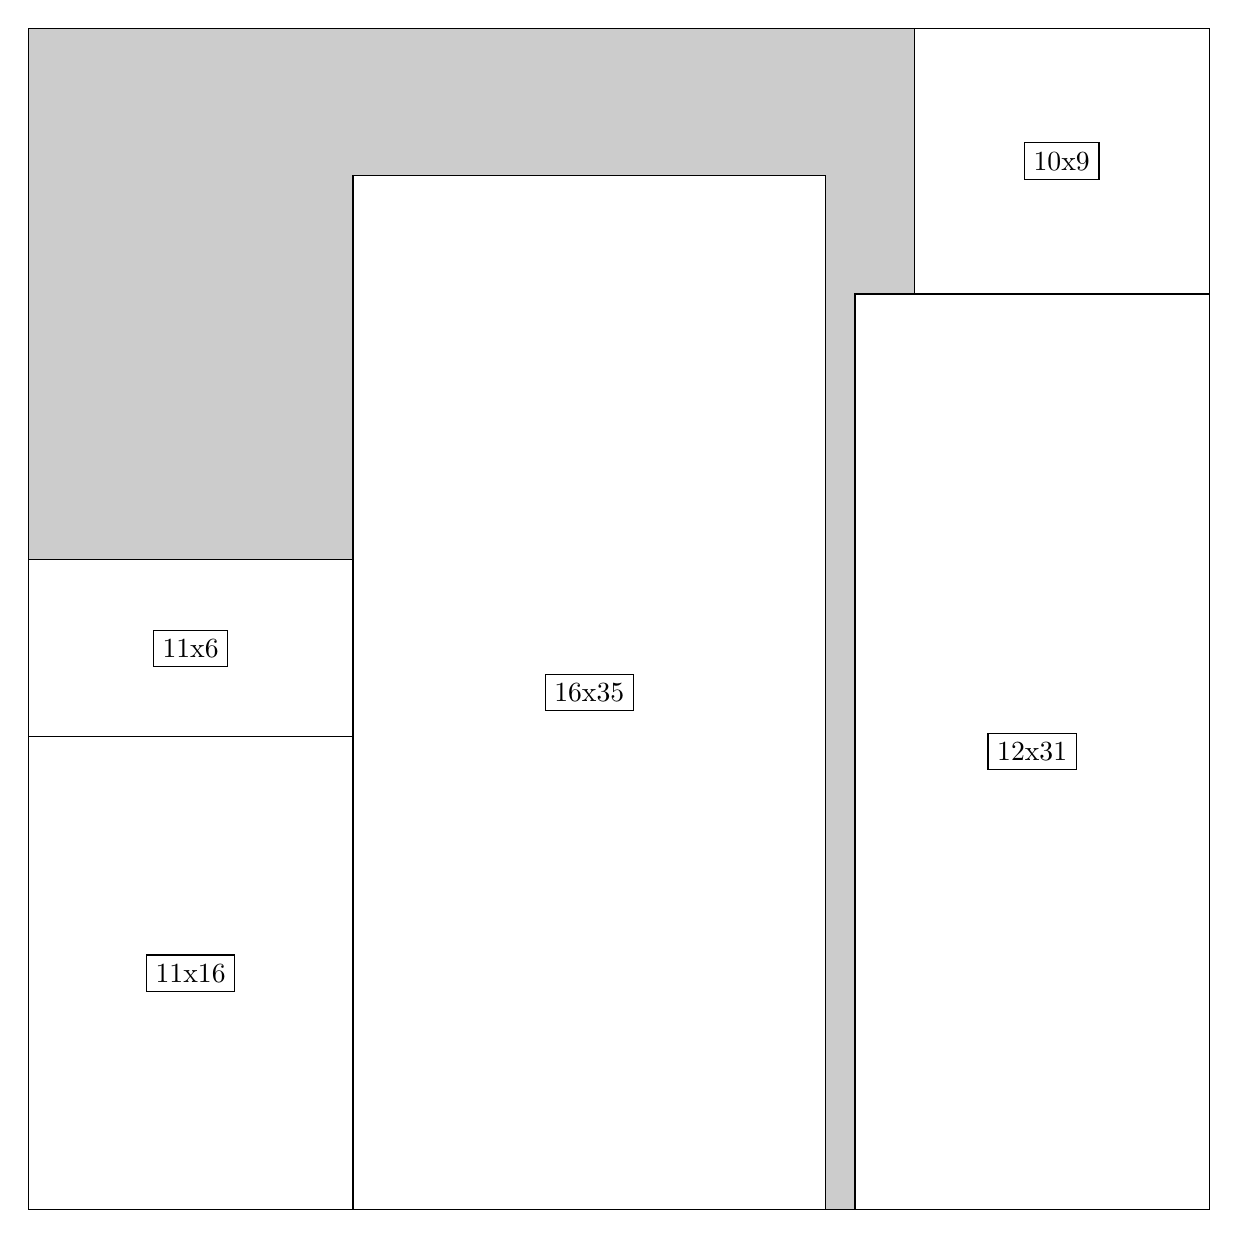
\begin{tikzpicture}[shorten >=1pt,scale=1.0,every node/.style={scale=1.0},->]
\tikzstyle{vertex}=[circle,fill=black!25,minimum size=14pt,inner sep=0pt]
\filldraw[fill=gray!40!white, draw=black] (0,0) rectangle (15.0,15.0);
\foreach \name/\x/\y/\w/\h in {12x31/10.5/0.0/4.5/11.625,10x9/11.25/11.625/3.75/3.375,16x35/4.125/0.0/6.0/13.125,11x16/0.0/0.0/4.125/6.0,11x6/0.0/6.0/4.125/2.25}
\filldraw[fill=white!40!white, draw=black] (\x,\y) rectangle node[draw] (\name) {\name} ++(\w,\h);
\end{tikzpicture}


w =12 , h =31 , x =28 , y =0 , v =372
\par
w =10 , h =9 , x =30 , y =31 , v =90
\par
w =16 , h =35 , x =11 , y =0 , v =560
\par
w =11 , h =16 , x =0 , y =0 , v =176
\par
w =11 , h =6 , x =0 , y =16 , v =66
\par
\newpage


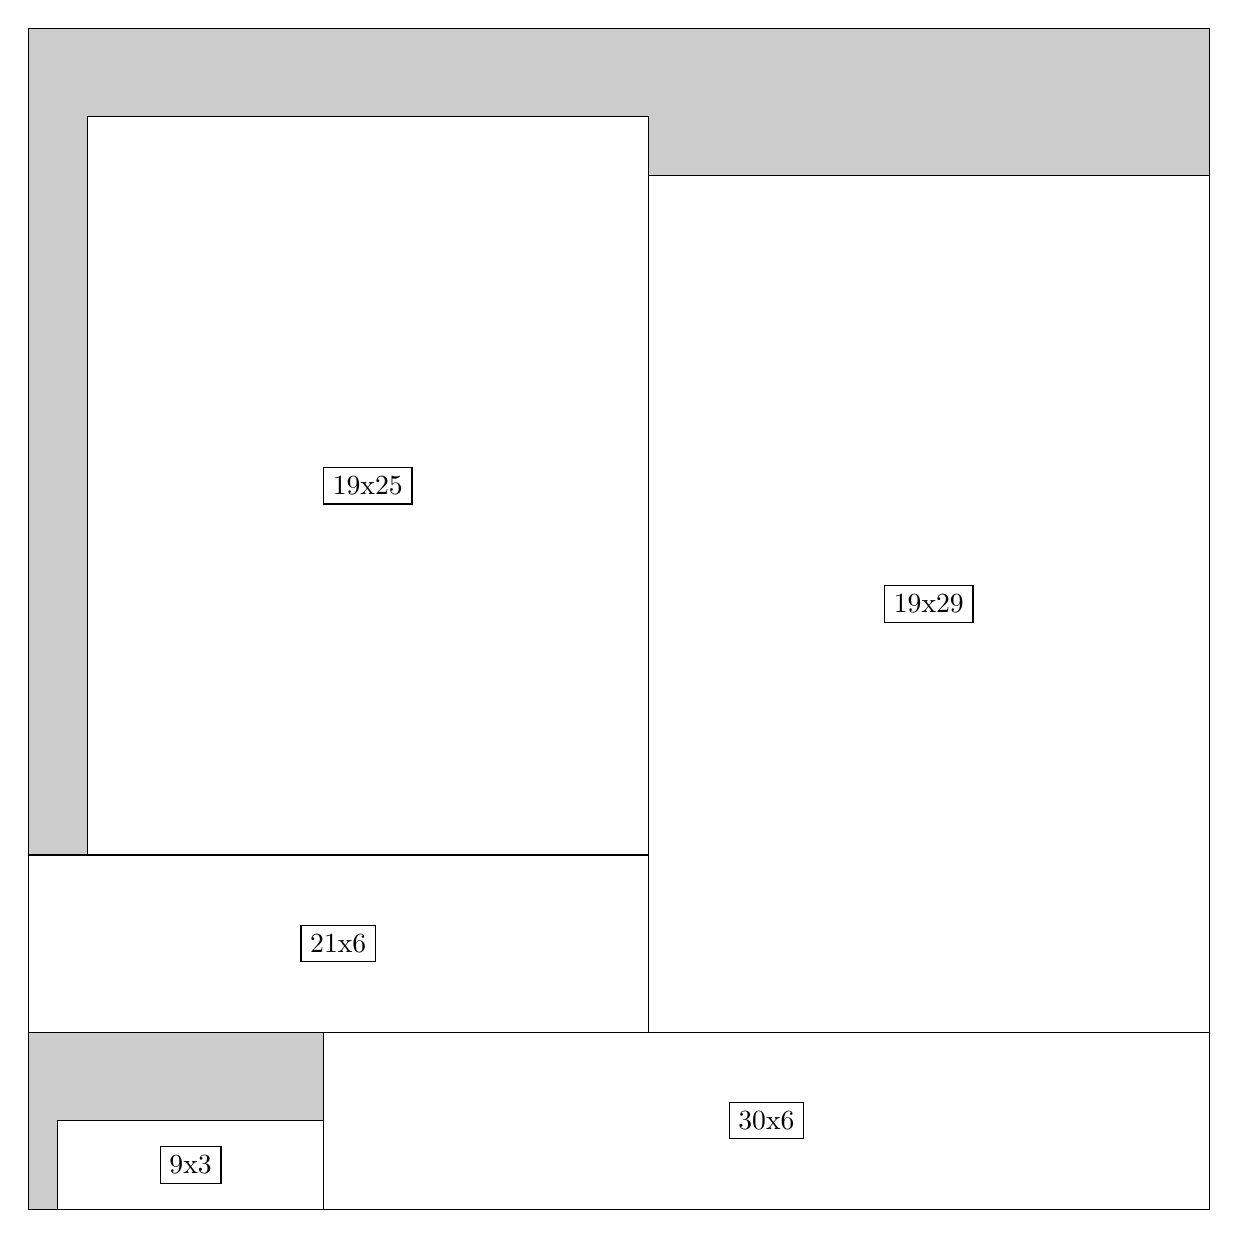
\begin{tikzpicture}[shorten >=1pt,scale=1.0,every node/.style={scale=1.0},->]
\tikzstyle{vertex}=[circle,fill=black!25,minimum size=14pt,inner sep=0pt]
\filldraw[fill=gray!40!white, draw=black] (0,0) rectangle (15.0,15.0);
\foreach \name/\x/\y/\w/\h in {30x6/3.75/0.0/11.25/2.25,9x3/0.375/0.0/3.375/1.125,19x29/7.875/2.25/7.125/10.875,21x6/0.0/2.25/7.875/2.25,19x25/0.75/4.5/7.125/9.375}
\filldraw[fill=white!40!white, draw=black] (\x,\y) rectangle node[draw] (\name) {\name} ++(\w,\h);
\end{tikzpicture}


w =30 , h =6 , x =10 , y =0 , v =180
\par
w =9 , h =3 , x =1 , y =0 , v =27
\par
w =19 , h =29 , x =21 , y =6 , v =551
\par
w =21 , h =6 , x =0 , y =6 , v =126
\par
w =19 , h =25 , x =2 , y =12 , v =475
\par
\newpage


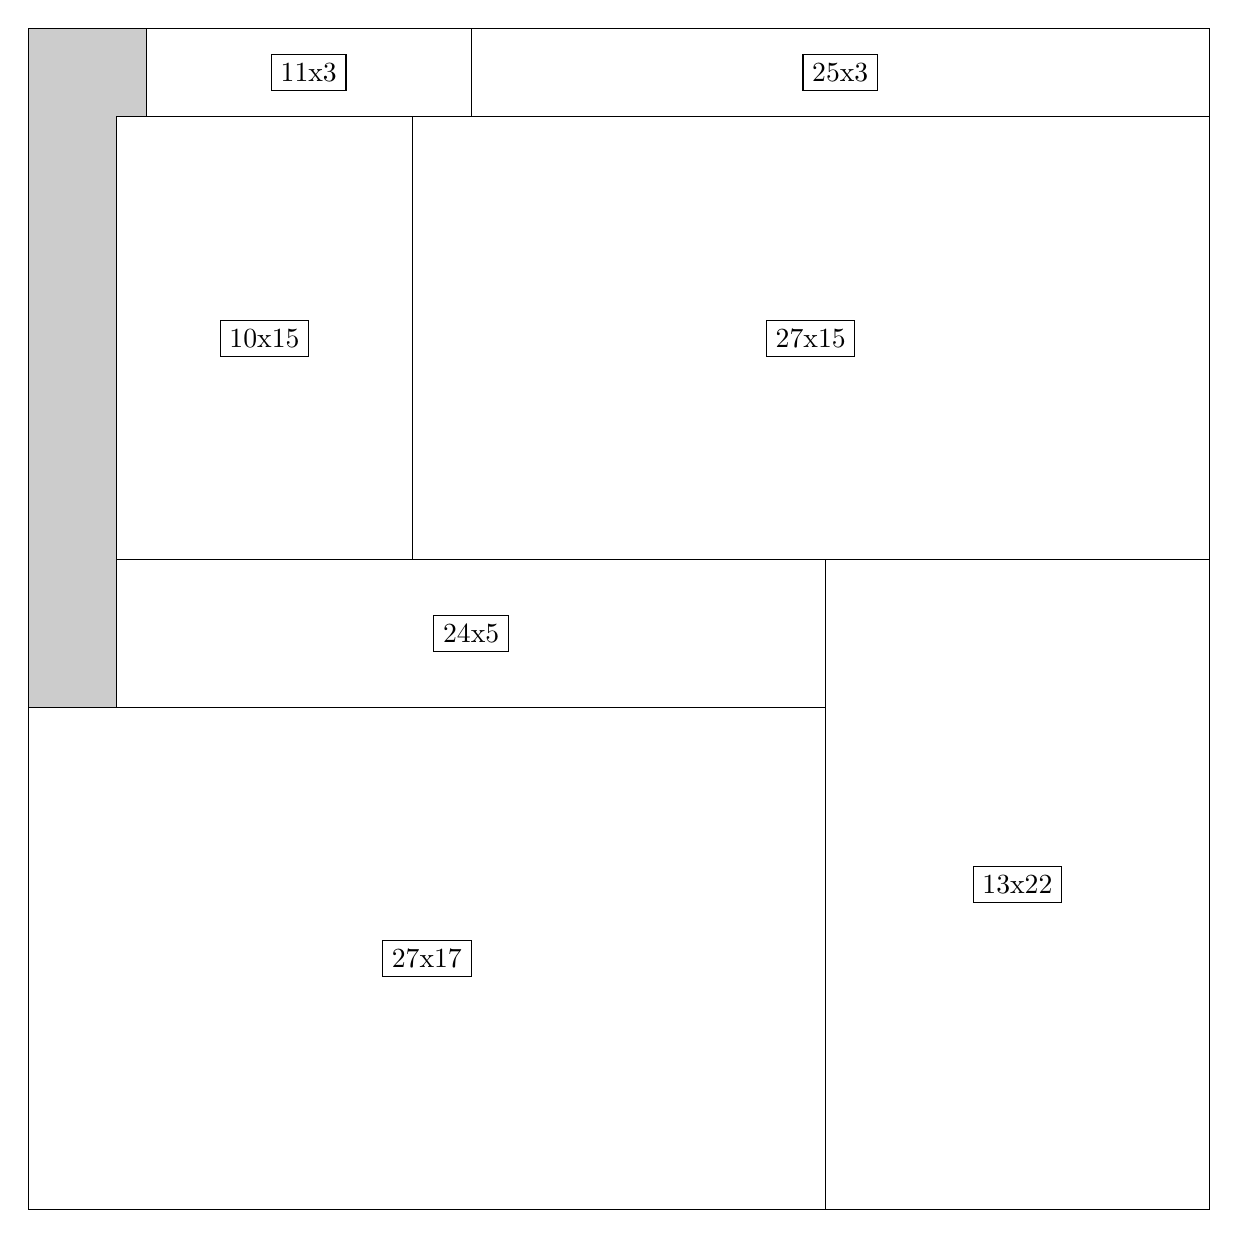
\begin{tikzpicture}[shorten >=1pt,scale=1.0,every node/.style={scale=1.0},->]
\tikzstyle{vertex}=[circle,fill=black!25,minimum size=14pt,inner sep=0pt]
\filldraw[fill=gray!40!white, draw=black] (0,0) rectangle (15.0,15.0);
\foreach \name/\x/\y/\w/\h in {13x22/10.125/0.0/4.875/8.25,27x17/0.0/0.0/10.125/6.375,24x5/1.125/6.375/9.0/1.875,27x15/4.875/8.25/10.125/5.625,10x15/1.125/8.25/3.75/5.625,25x3/5.625/13.875/9.375/1.125,11x3/1.5/13.875/4.125/1.125}
\filldraw[fill=white!40!white, draw=black] (\x,\y) rectangle node[draw] (\name) {\name} ++(\w,\h);
\end{tikzpicture}


w =13 , h =22 , x =27 , y =0 , v =286
\par
w =27 , h =17 , x =0 , y =0 , v =459
\par
w =24 , h =5 , x =3 , y =17 , v =120
\par
w =27 , h =15 , x =13 , y =22 , v =405
\par
w =10 , h =15 , x =3 , y =22 , v =150
\par
w =25 , h =3 , x =15 , y =37 , v =75
\par
w =11 , h =3 , x =4 , y =37 , v =33
\par
\newpage


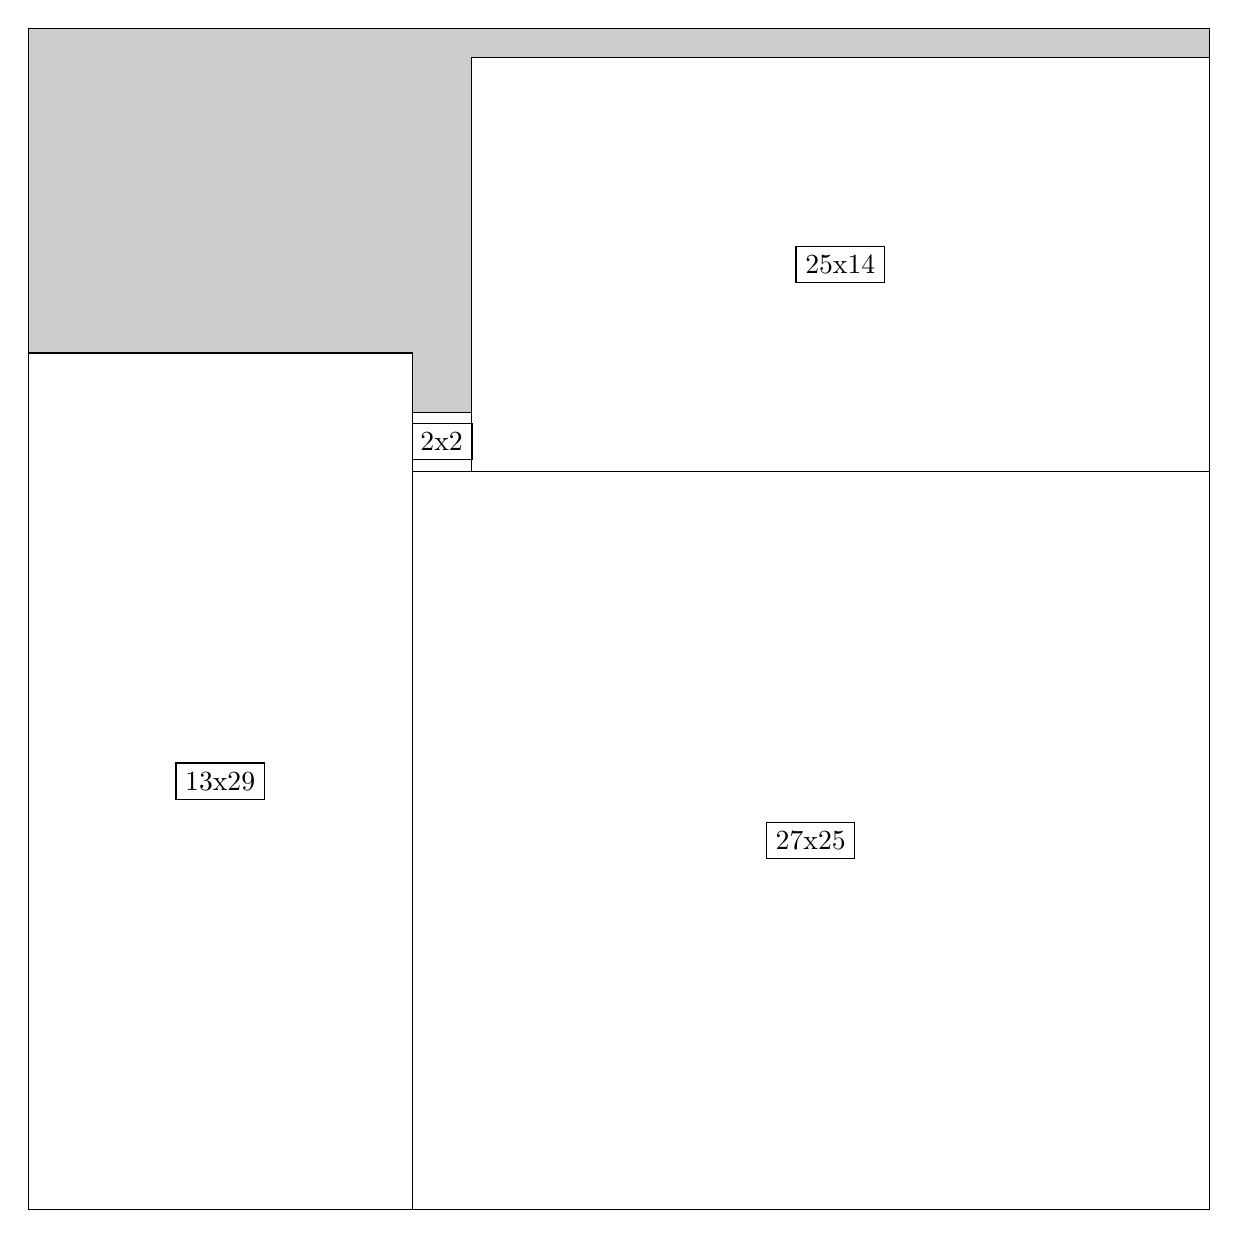
\begin{tikzpicture}[shorten >=1pt,scale=1.0,every node/.style={scale=1.0},->]
\tikzstyle{vertex}=[circle,fill=black!25,minimum size=14pt,inner sep=0pt]
\filldraw[fill=gray!40!white, draw=black] (0,0) rectangle (15.0,15.0);
\foreach \name/\x/\y/\w/\h in {27x25/4.875/0.0/10.125/9.375,25x14/5.625/9.375/9.375/5.25,2x2/4.875/9.375/0.75/0.75,13x29/0.0/0.0/4.875/10.875}
\filldraw[fill=white!40!white, draw=black] (\x,\y) rectangle node[draw] (\name) {\name} ++(\w,\h);
\end{tikzpicture}


w =27 , h =25 , x =13 , y =0 , v =675
\par
w =25 , h =14 , x =15 , y =25 , v =350
\par
w =2 , h =2 , x =13 , y =25 , v =4
\par
w =13 , h =29 , x =0 , y =0 , v =377
\par
\newpage


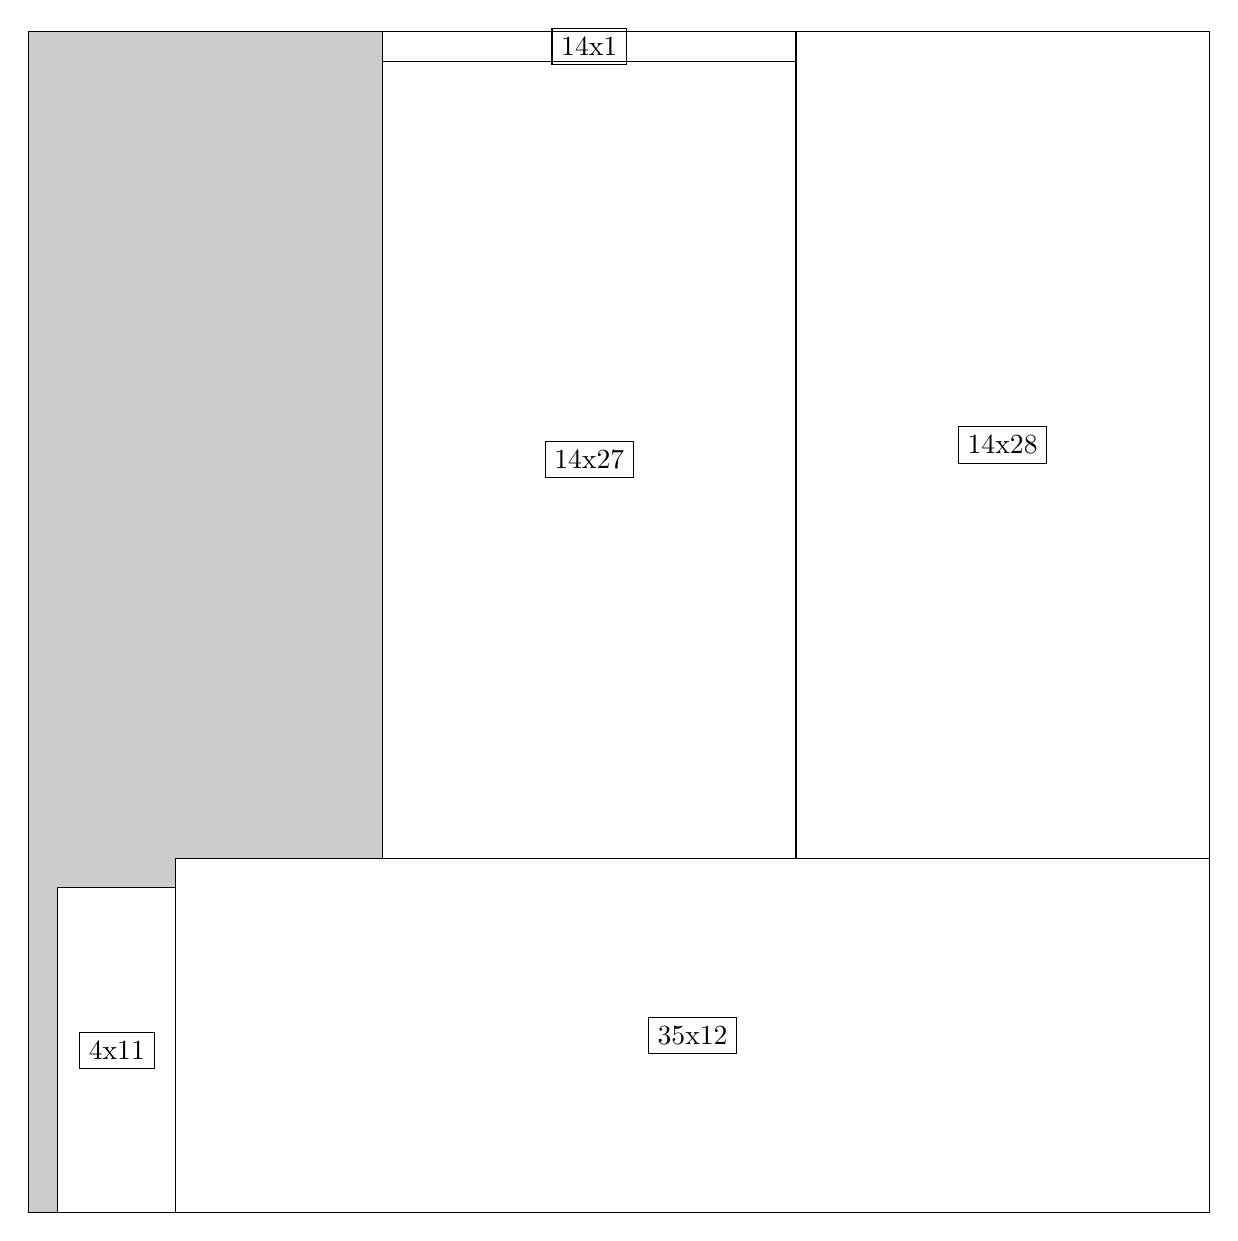
\begin{tikzpicture}[shorten >=1pt,scale=1.0,every node/.style={scale=1.0},->]
\tikzstyle{vertex}=[circle,fill=black!25,minimum size=14pt,inner sep=0pt]
\filldraw[fill=gray!40!white, draw=black] (0,0) rectangle (15.0,15.0);
\foreach \name/\x/\y/\w/\h in {35x12/1.875/0.0/13.125/4.5,4x11/0.375/0.0/1.5/4.125,14x28/9.75/4.5/5.25/10.5,14x27/4.5/4.5/5.25/10.125,14x1/4.5/14.625/5.25/0.375}
\filldraw[fill=white!40!white, draw=black] (\x,\y) rectangle node[draw] (\name) {\name} ++(\w,\h);
\end{tikzpicture}


w =35 , h =12 , x =5 , y =0 , v =420
\par
w =4 , h =11 , x =1 , y =0 , v =44
\par
w =14 , h =28 , x =26 , y =12 , v =392
\par
w =14 , h =27 , x =12 , y =12 , v =378
\par
w =14 , h =1 , x =12 , y =39 , v =14
\par
\newpage


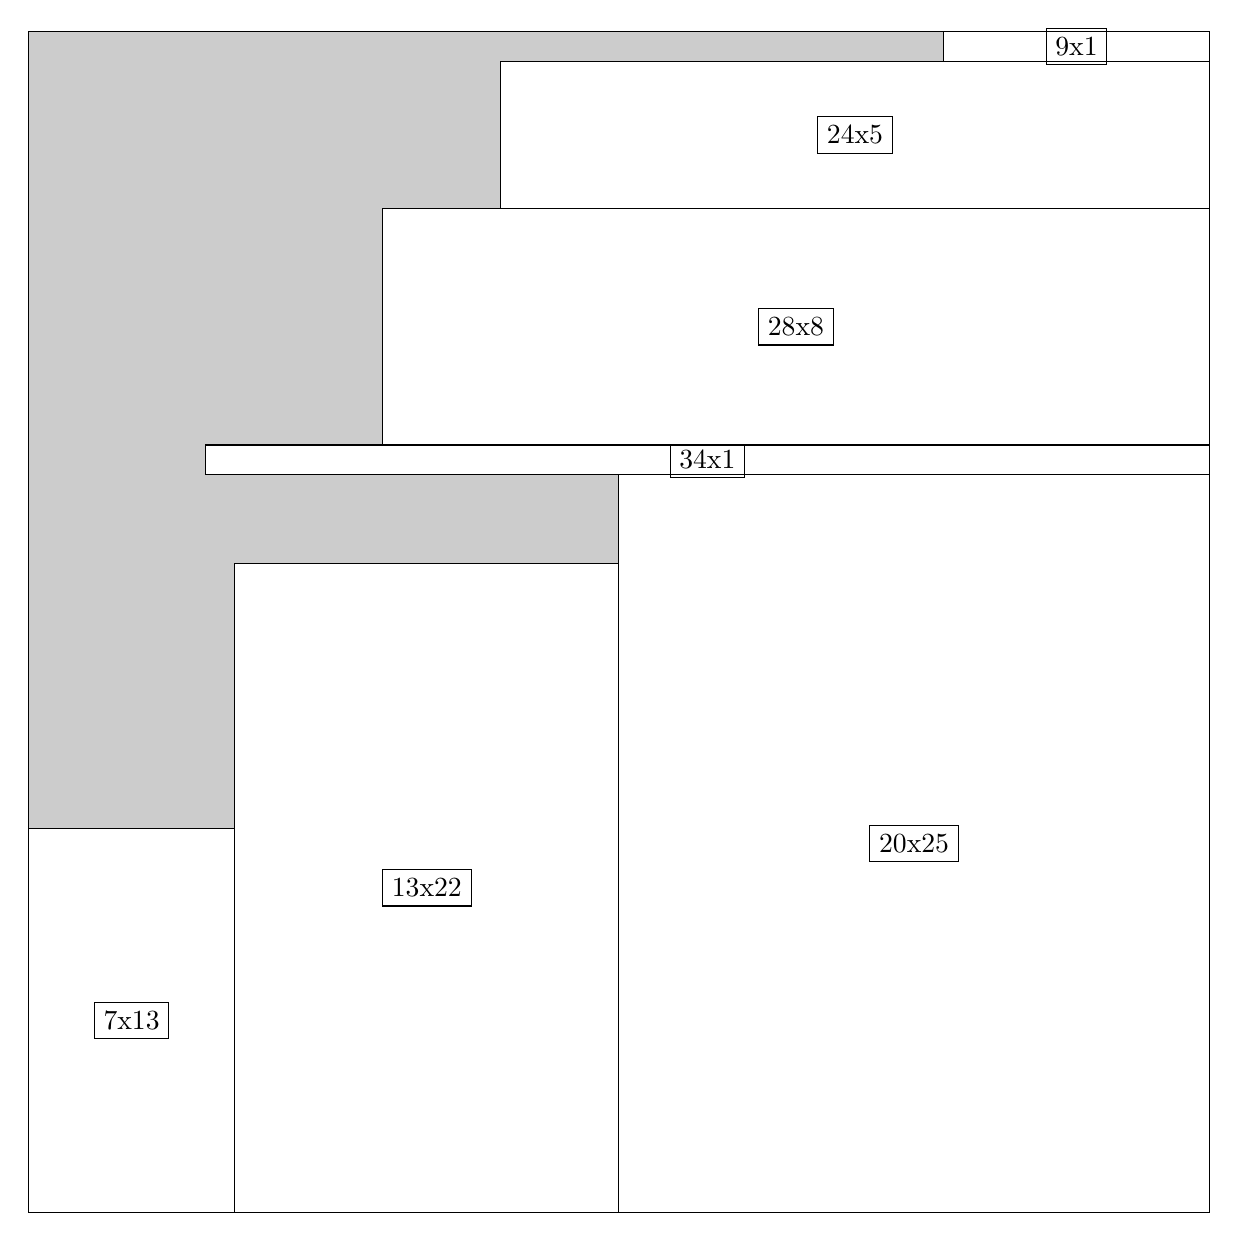
\begin{tikzpicture}[shorten >=1pt,scale=1.0,every node/.style={scale=1.0},->]
\tikzstyle{vertex}=[circle,fill=black!25,minimum size=14pt,inner sep=0pt]
\filldraw[fill=gray!40!white, draw=black] (0,0) rectangle (15.0,15.0);
\foreach \name/\x/\y/\w/\h in {20x25/7.5/0.0/7.5/9.375,13x22/2.625/0.0/4.875/8.25,7x13/0.0/0.0/2.625/4.875,34x1/2.25/9.375/12.75/0.375,28x8/4.5/9.75/10.5/3.0,24x5/6.0/12.75/9.0/1.875,9x1/11.625/14.625/3.375/0.375}
\filldraw[fill=white!40!white, draw=black] (\x,\y) rectangle node[draw] (\name) {\name} ++(\w,\h);
\end{tikzpicture}


w =20 , h =25 , x =20 , y =0 , v =500
\par
w =13 , h =22 , x =7 , y =0 , v =286
\par
w =7 , h =13 , x =0 , y =0 , v =91
\par
w =34 , h =1 , x =6 , y =25 , v =34
\par
w =28 , h =8 , x =12 , y =26 , v =224
\par
w =24 , h =5 , x =16 , y =34 , v =120
\par
w =9 , h =1 , x =31 , y =39 , v =9
\par
\newpage


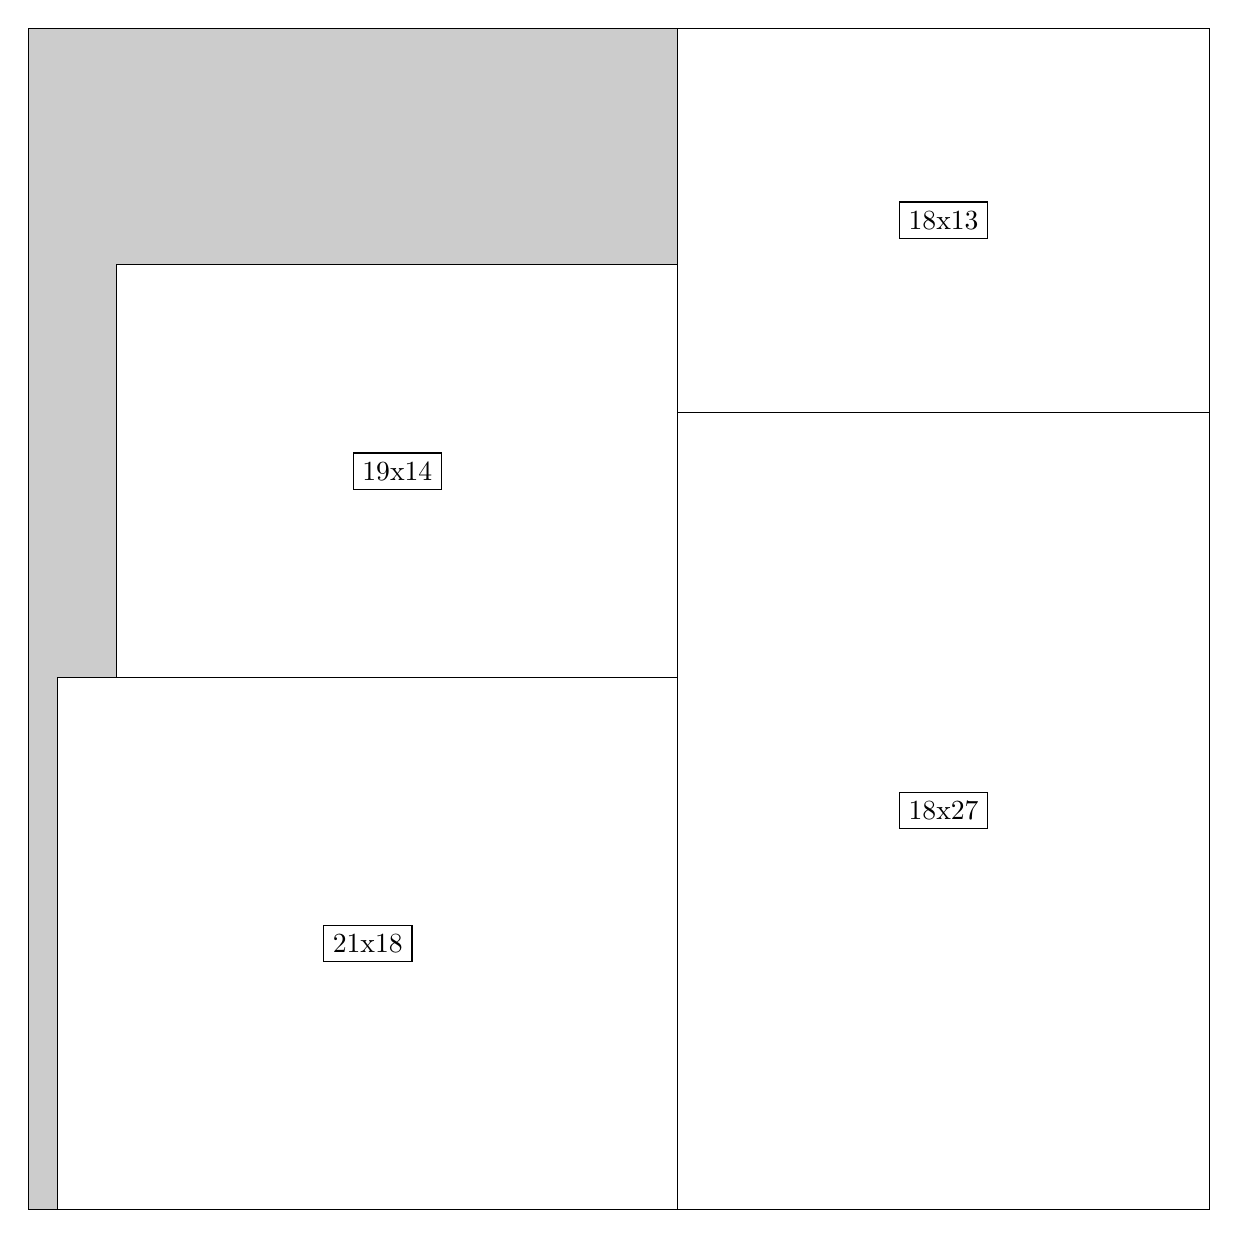
\begin{tikzpicture}[shorten >=1pt,scale=1.0,every node/.style={scale=1.0},->]
\tikzstyle{vertex}=[circle,fill=black!25,minimum size=14pt,inner sep=0pt]
\filldraw[fill=gray!40!white, draw=black] (0,0) rectangle (15.0,15.0);
\foreach \name/\x/\y/\w/\h in {18x27/8.25/0.0/6.75/10.125,18x13/8.25/10.125/6.75/4.875,21x18/0.375/0.0/7.875/6.75,19x14/1.125/6.75/7.125/5.25}
\filldraw[fill=white!40!white, draw=black] (\x,\y) rectangle node[draw] (\name) {\name} ++(\w,\h);
\end{tikzpicture}


w =18 , h =27 , x =22 , y =0 , v =486
\par
w =18 , h =13 , x =22 , y =27 , v =234
\par
w =21 , h =18 , x =1 , y =0 , v =378
\par
w =19 , h =14 , x =3 , y =18 , v =266
\par
\newpage


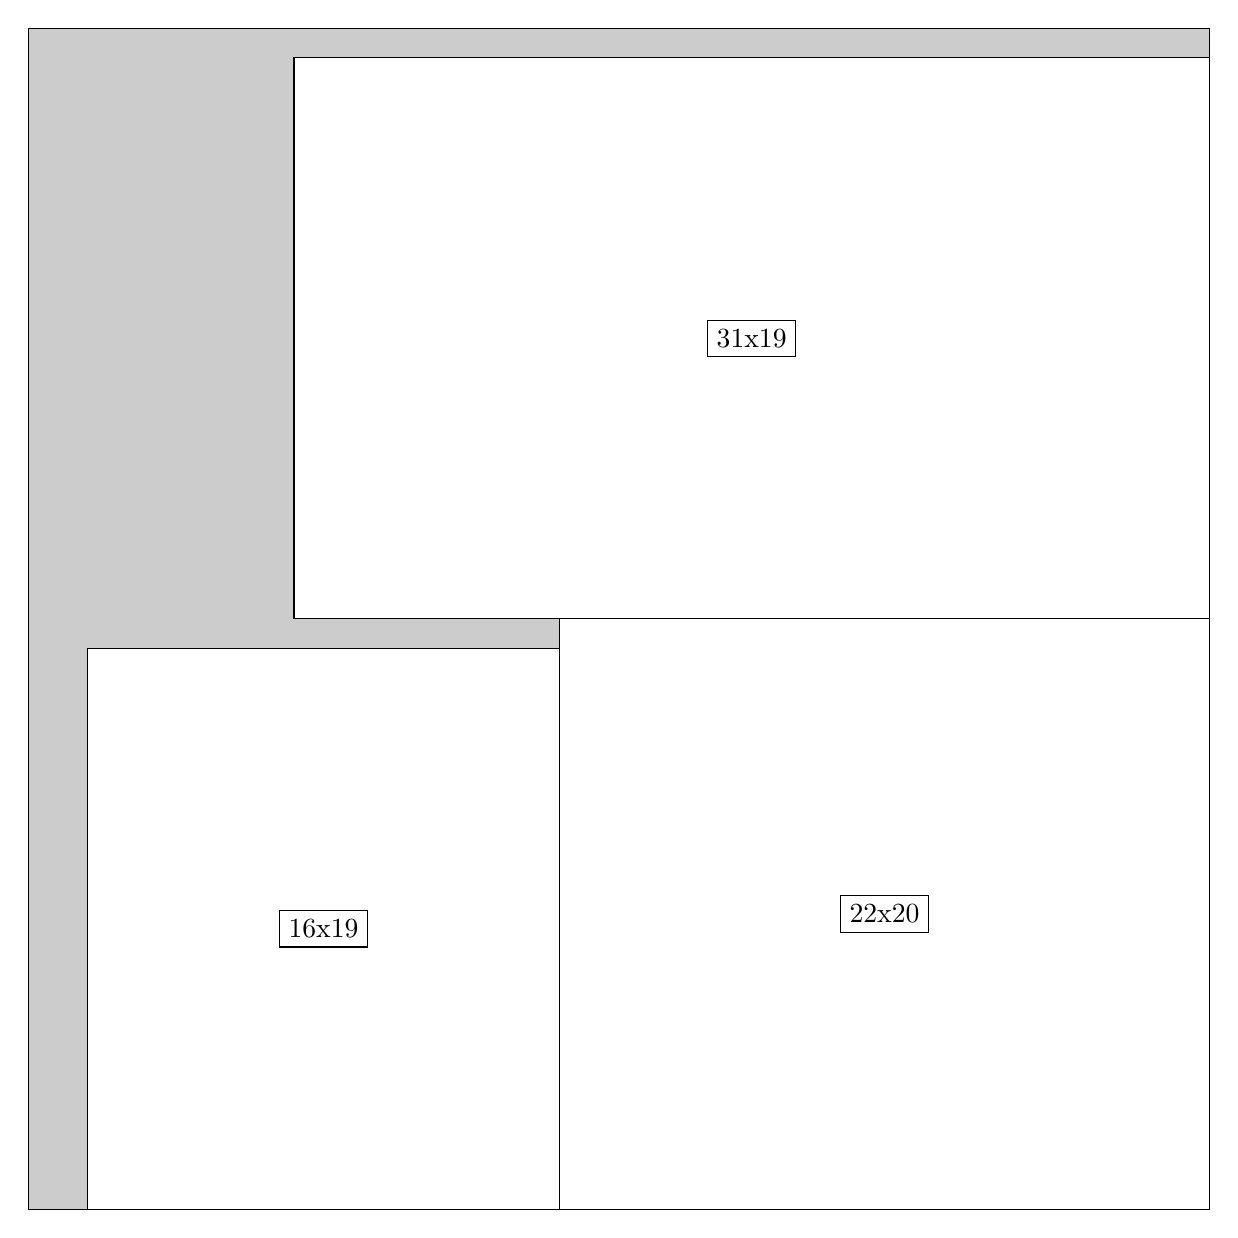
\begin{tikzpicture}[shorten >=1pt,scale=1.0,every node/.style={scale=1.0},->]
\tikzstyle{vertex}=[circle,fill=black!25,minimum size=14pt,inner sep=0pt]
\filldraw[fill=gray!40!white, draw=black] (0,0) rectangle (15.0,15.0);
\foreach \name/\x/\y/\w/\h in {22x20/6.75/0.0/8.25/7.5,16x19/0.75/0.0/6.0/7.125,31x19/3.375/7.5/11.625/7.125}
\filldraw[fill=white!40!white, draw=black] (\x,\y) rectangle node[draw] (\name) {\name} ++(\w,\h);
\end{tikzpicture}


w =22 , h =20 , x =18 , y =0 , v =440
\par
w =16 , h =19 , x =2 , y =0 , v =304
\par
w =31 , h =19 , x =9 , y =20 , v =589
\par
\newpage


\end{document}